\section{Description of the server}
\label{sec:Description of the server}

We implemented our server in Java. Our server receives request and if it is busy proccessing one,
coming request will be added to the queue and proccessed later. The server can be either
single threaded (SimpleServer.java) meaning that it can only process one request at a time. Or
it can use multiple thread(ThreadedServer.java) to process several requests at the same time.

\subsection{Computation performed by the server}
\label{sub:Computation performed by the server}
The compution performed by the server consist of calculating the power of a
two-dimensional Matrix $M$ powered by a natural $p$.

\subsection{Request and response format}
\label{sub:Request and response format}

Each client request contains the matrix and the exposant. To achieve the
measurement that were asked, we added some fields to the request to get
some information such as computation time and and response time. We also
give an identifier to a request to make a mapping between request and response.

\section{Description of the measurement setup}
\label{sec:Description of the measurement setup}

\subsection{Used hardwares and softwares}
\label{sub:Used hardwares and softwares}

For our tests, two computer from the Intel room were used (in the Reaumur
building), they have the following specifications :

\begin{tabular}{|l|l|}
    \hline
    Processor & Intel(R) Core(TM)2 Quad Q6600 \@ 2.40GHz \\
    Instruction set & 64-bit \\
    \hline
    Total memory & 3981192 kB \\
    Total swap & 4063228 kB \\
    \hline
    Ethernet controller: Intel Corporation 82566DM-2 Gigabit Network Connection
    \hline
\end{tabular}
\bigskip

Those computers run on Linux (centOS distribution) so we used \enquote{top},
\enquote{htop} and \nequote{grep} to monitor CPU load and \enquote{Wireshark}
to monitor network usage (because nor \enquote{NetHogs} nor \enquote{iftop} were
installed). \newline

\subsection{Description of the load generator}
\label{sub:Description of the load generator}
We implemented a LoadGenerator to simulate the behavior of many independent
clients. The LoadGenerator uses the inversion method to generate exponentiallly
distributed randoms numbers to create inter-request times.

\section{Measurements and modeling}
\label{sec:Measurements and modeling}

\subsection{Measurement of individual client requests}
\label{sub:Measurement of individual client requests}

The figure~\ref{fig:measurement1} shows the evolution of the average time needed
according to size-changing matrices. For the lower sized matrices, the network
time is the most impactful factor on the average time. The network time is

\begin{figure}[!ht]
    \centering
    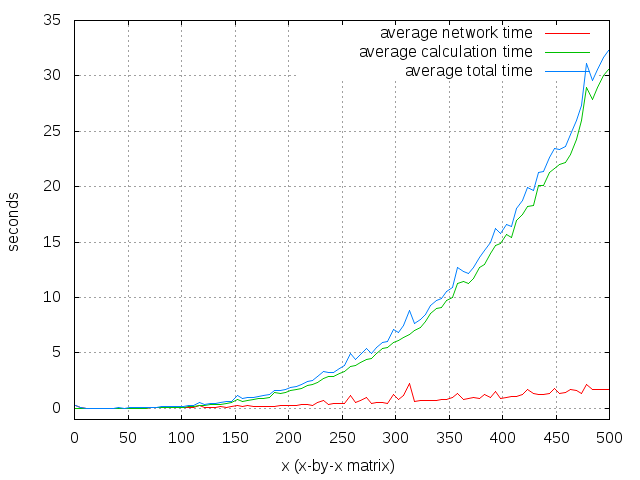
\includegraphics[width=\linewidth]{measurement1.png}
    \caption{Measurement of average time needed depending on size-changing matrices}
    \label{fig:measurement1}
\end{figure}

\subsection{Measurement of the load generator}
\label{sub:Measurement of the load generator}

\subsection{Queueing station model}
\label{sub:Queueing station model}

\subsection{Improvement of the performance of the system}
\label{sub:Improvement of the performance of the system}

\subsection{Measurements on a multi-threaded server}
\label{sub:Measurements on a multi-threaded server}

\subsubsection{Bottlenecks}
\label{subs:Bottlenecks}


\subsubsection{Multi-threading and queuing station model}
\label{subs:Multi-threading and queuing station model}
